\documentclass[reprint,pra, twocolumn, amsmath,amssymb,
 aps,superscriptaddress,]{revtex4-2}

\usepackage[utf8]{inputenc}
\usepackage[english]{babel}
\usepackage[a4paper,margin=2.0cm]{geometry}

\makeatletter
\setlength{\@fptop}{0pt}
\makeatother

\columnsep=1.0pc
\parindent=1.0cm
\parskip=6.0pt
\usepackage{amsmath,amsfonts,amssymb,dsfont,amsthm}
\usepackage{indentfirst}
\usepackage{graphicx}
\usepackage{booktabs}
\usepackage{siunitx}
\usepackage{lipsum}
\usepackage{listings}
\sisetup{output-decimal-marker={,}}
\sisetup{use-xspace}
\sisetup{space-before-unit}
\sisetup{angle-symbol-over-decimal}
\sisetup{group-digits=false}
\DeclareMathOperator{\Tr}{Tr}
\usepackage{tasks}
\usepackage{amssymb}
%\usepackage{wasysym}
\usepackage[T1]{fontenc}
%\usepackage{authblk}
%\usepackage[raggedright]{titlesec}

\usepackage{comment}
\usepackage{mathtools}
\usepackage{extpfeil}
\usepackage{xcolor}
\usepackage{hyperref}
\usepackage{url}
\usepackage{natbib}
\usepackage{makecell}

\usepackage{physics}
%\AtBeginDocument{\RenewCommandCopy\qty\SI}
\usepackage{graphicx}% Include figure files
\usepackage{dcolumn}% Align table columns on decimal point
\usepackage{bm}% bold math
\usepackage{tikz}
\usepackage{pgf}
\usepackage{tikzscale}
\usetikzlibrary{angles,calc,intersections,quotes,arrows.meta, shapes,decorations.markings, external}
%\tikzexternalize


\newtheorem{thm}{Theorem}%[section]
\newtheorem{lem}{Lemma}
\newtheorem{prop}{Proposition}
\newtheorem{cor}{Corollary}
\newtheorem{defi}{Definition}
\newtheorem{rem}{Remark}
\newtheorem{ex}{Exercise}
\newtheorem{eg}{Example}
\newtheorem{obs}{Observation}

\newcommand{\ie}{\textit{i.e.}}
\newcommand{\eq}{Eq.}
\newcommand{\muns}{$\mu^{\text{NS}}$}
\newcommand{\alice}{$\mathcal{A}$}
\newcommand{\bob}{$\mathcal{B}$}

\newcommand{\noob}[1]{\textcolor{blue}{[A:#1]}}
\newcommand{\lu}[1]{\textcolor{red}{[L:#1]}}

\newcommand{\ba}[1]{\begin{align} #1 \end{align}}
\newcommand{\bfr}[2]{\begin{frame}{#1} #2 \end{frame}}
\newcommand{\bi}[1]{\begin{itemize} #1 \end{itemize}}
\newcommand{\be}[1]{\begin{enumerate} #1 \end{enumerate}}
\newcommand{\beq}[1]{\begin{equation} #1 \end{equation}}
\newtheorem{lemma}{Lemma}
\newtheorem{result}{Result}




\date{May 2026}

\begin{document}

\title{The entropic approach for quantum networks: Notes}

\author{}
\email{}
\affiliation{}

\maketitle
\onecolumngrid
\section{Introduction}
Quantum mechanics admits correlations among spatially separated parties that cannot be reproduced by any classical model based on shared common causes.
Bell's theorem establishes this in its simplest form: two parties share a source, each chooses among incompatible measurements, and the resulting correlations can violate the constraints implied by any local hidden-variable model \cite{Bell64}.
More recently, this has been generalised to \emph{networks}: causal structures in which several independent sources jointly distribute correlations among multiple observed parties \cite{HensonLalPusey,Fritz,Branciard2010Bilocality}.
Such networks support genuinely novel forms of nonclassicality, distinct from the bipartite case and not necessarily reducible to a standard Bell violation \cite{Renou2019triangle}. 
This generalisation, however, comes at a structural cost.
When considering probability distributions, the independence of the sources requirement renders the set of classically realisable correlations non-convex in general.
Therefore, the convex-polytope machinery that underlies the standard Bell-nonclassicality program does not transfer directly.
Two distinct attempts to recover such a framework have emerged.


The first attempt employs the entropic formulation of Bell inequalities \cite{BraunsteinCaves88,CerfAdami97}.
Its applicability to networks was recognised later \cite{FritzChaves13,ChavesLuftGross14,WeilenmannColbeck17}.
When considering entropies, the multiplicative source-independence constraint becomes an additive equality.
The non-convexity of the probability description is thereby linearised, rendering the cone of joint Shannon entropies a tractable object of study for causal compatibility in networks.
The second attempt is that of the \emph{inflation technique} \cite{WolfeSpekkensFritz19}.
The original network is replaced by a strictly larger causal structure containing copies of the sources and observed variables present in the original causal structure, in which any classical realisation of the original must extend to the inflated structure.
The inflated structure admits additional independence relations, whose consequences on the observed marginals yield stronger compatibility tests.
Inflation has since become the most successful structural device for tightening tests of network nonclassicality.

These two attempts have developed largely in parallel. In this work, we consider how these two techniques may be combined.

\section{The triangle network}

\begin{figure}[t]
    \centering
    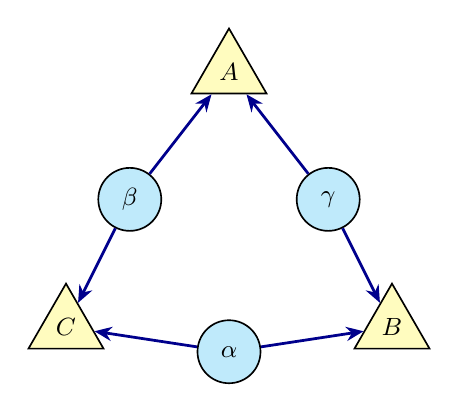
\begin{tikzpicture}[
        scale=0.9,
        observed/.style={
            regular polygon, regular polygon sides=3,
            draw=black, fill=yellow!25, line width=0.6pt,
            inner sep=1pt, minimum size=11mm,
            font=\small
        },
        source/.style={
            circle, draw=black, fill=cyan!25, line width=0.6pt,
            inner sep=1pt, minimum size=8mm,
            font=\small
        },
        arr/.style={
            -{Stealth[length=2.2mm,width=1.8mm]},
            line width=1.0pt, color=blue!55!black
        }
    ]
        \node[observed] (A) at (0, 2.4) {$A$};
        \node[observed] (B) at (2.3, -1.2) {$B$};
        \node[observed] (C) at (-2.3, -1.2) {$C$};

        \node[source] (beta)  at (-1.4, 0.6) {$\beta$};
        \node[source] (gamma) at (1.4, 0.6) {$\gamma$};
        \node[source] (alpha) at (0, -1.55) {$\alpha$};

        \draw[arr] (beta)  -- (A);
        \draw[arr] (beta)  -- (C);
        \draw[arr] (gamma) -- (A);
        \draw[arr] (gamma) -- (B);
        \draw[arr] (alpha) -- (B);
        \draw[arr] (alpha) -- (C);
    \end{tikzpicture}
    \caption{The triangle network. Three observed parties $A$, $B$, $C$ are pairwise connected by three independent latent sources $\alpha$, $\beta$, $\gamma$.}
    \label{fig:triangle}
\end{figure}

We consider the \emph{triangle network}, depicted in Fig.~\ref{fig:triangle}.
It consists of three observed parties, $A$, $B$, and $C$, pairwise connected by three independent latent sources $\alpha$, $\beta$, and $\gamma$.
The source $\alpha$ is a common cause for $B$ and $C$; $\beta$ for $A$ and $C$; and $\gamma$ for $A$ and $B$.
The three sources are mutually independent.
Unlike the standard Bell scenario, no measurement settings are involved: each party performs a single fixed measurement on the systems it receives.

If we consider the random variables $A$, $B$, $C$, $\alpha$, $\beta$, $\gamma$ and the relations imposed on them by the causal structure, we can define a corresponding Shannon-type cone encoding constraints on their joint entropies $H(\cdot)$.
These constraints impose non-trivial consequences on the observed variables $A$, $B$, $C$.
Projecting the cone onto the observed entropy coordinates $\{H(A), H(B), H(C), H(A,B), H(A,C), H(B,C), H(A,B,C)\}$ yields a finite family of linear inequalities that every classical realisation of the triangle must satisfy.
For the triangle, this projection is known explicitly: it consists of seven inequalities \cite{ChavesLuftGross14}, organised in three symmetry classes under cyclic permutation of the parties.
The three representatives are
\begin{align}
    H(A,B) + H(A,C) &\geq H(A) + H(B) + H(C), \label{ineq:triangle1} \\
    4\,[H(A,B) + H(A,C) + H(B,C)] &\geq 5\,[H(A) + H(B) + H(C)] + 2\,H(A,B,C), \label{ineq:triangle2} \\
    3\,H(A,B) + 2\,H(A,C) + 2\,H(B,C) &\geq 3\,[H(A) + H(B) + H(C)] + H(A,B,C). \label{ineq:triangle3}
\end{align}
The first and third generate two further inequalities each under cyclic permutation of $A$, $B$, $C$; the second is fully symmetric.

Note that these seven inequalities further constrain the set of entropy vectors already allowed by the basic Shannon-type constraints over $A$, $B$, $C$ alone.
In the entropy basis $\{H(A), H(B), H(C), H(A,B), H(A,C), H(B,C), H(A,B,C)\}$ the latter are the nine elemental inequalities encoding non-negativity of each conditional entropy $H(X_i \mid X_j, X_k)$ and of each conditional mutual information $I(X_i ; X_j \mid X_k)$.
The polyhedral cone they define admits an equivalent description as the conic hull of a finite set of extreme rays, listed in Table~\ref{tab:shannon-rays}.
Of these eight rays, the fully symmetric one $r_1 = (1,1,1,1,1,1,1)$ violates all seven triangle inequalities, confirming that the triangle inequalities cut strictly into the basic Shannon cone.

\begin{table}[h]
    \centering
    \begin{tabular}{c|ccccccc}
        & $H(A)$ & $H(B)$ & $H(C)$ & $H(A,B)$ & $H(A,C)$ & $H(B,C)$ & $H(A,B,C)$ \\
        \hline
        $r_0$ & 1 & 1 & 0 & 1 & 1 & 1 & 1 \\
        $r_1$ & 1 & 1 & 1 & 1 & 1 & 1 & 1 \\
        $r_2$ & 1 & 1 & 1 & 2 & 2 & 2 & 2 \\
        $r_3$ & 1 & 0 & 1 & 1 & 1 & 1 & 1 \\
        $r_4$ & 0 & 1 & 1 & 1 & 1 & 1 & 1 \\
        $r_5$ & 0 & 0 & 1 & 0 & 1 & 1 & 1 \\
        $r_6$ & 0 & 1 & 0 & 1 & 0 & 1 & 1 \\
        $r_7$ & 1 & 0 & 0 & 1 & 1 & 0 & 1 \\
    \end{tabular}
    \caption{Extreme rays of the basic Shannon cone for three random variables $A$, $B$, $C$. Of the eight rays, only $r_1$ violates the triangle inequalities; all others satisfy them.}
    \label{tab:shannon-rays}
\end{table}

Combining the seven triangle inequalities with the basic Shannon-type constraints yields an outer approximation of the cone of entropy vectors realisable in the triangle causal structure.
This combined cone also admits a finite description in terms of its extreme rays, listed in Table~\ref{tab:triangle-rays}.
By construction, each of these rays satisfies every inequality currently known for the triangle scenario.

\begin{table}[h]
    \centering
    \begin{tabular}{c|ccccccc}
        & $H(A)$ & $H(B)$ & $H(C)$ & $H(A,B)$ & $H(A,C)$ & $H(B,C)$ & $H(A,B,C)$ \\
        \hline
        $r_0$ & 1   & 1   & 0   & 1   & 1   & 1   & 1 \\
        $r_1$ & 1   & 1.5 & 1.5 & 2   & 2   & 2.5 & 3 \\
        $r_2$ & 1.5 & 1   & 1.5 & 2   & 2.5 & 2   & 3 \\
        $r_3$ & 1.5 & 1.5 & 1   & 2.5 & 2   & 2   & 3 \\
        $r_4$ & 1   & 1   & 1   & 2   & 2   & 2   & 2 \\
        $r_5$ & 1   & 0   & 1   & 1   & 1   & 1   & 1 \\
        $r_6$ & 1   & 0   & 0   & 1   & 1   & 0   & 1 \\
        $r_7$ & 0   & 1   & 1   & 1   & 1   & 1   & 1 \\
        $r_8$ & 0   & 1   & 0   & 1   & 0   & 1   & 1 \\
        $r_9$ & 0   & 0   & 1   & 0   & 1   & 1   & 1 \\
    \end{tabular}
    \caption{Extreme rays of the outer approximation of the triangle entropy cone, defined by the basic Shannon-type constraints together with the seven triangle inequalities. All ten rays satisfy every inequality currently known for the triangle scenario.}
    \label{tab:triangle-rays}
\end{table}

\section{The spiral inflation}

\begin{figure}[t]
    \centering
    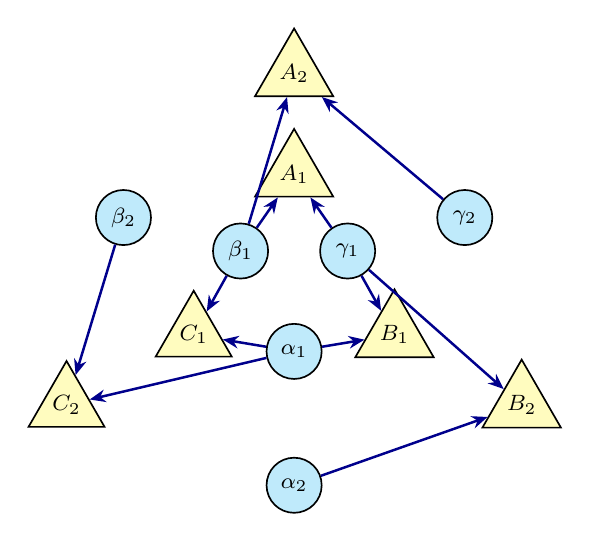
\begin{tikzpicture}[
        scale=0.85,
        observed/.style={
            regular polygon, regular polygon sides=3,
            draw=black, fill=yellow!25, line width=0.6pt,
            inner sep=0.5pt, minimum size=9mm,
            font=\footnotesize
        },
        source/.style={
            circle, draw=black, fill=cyan!25, line width=0.6pt,
            inner sep=0.5pt, minimum size=7mm,
            font=\footnotesize
        },
        arr/.style={
            -{Stealth[length=2mm,width=1.6mm]},
            line width=0.9pt, color=blue!55!black
        }
    ]
        % Inner parties
        \node[observed] (A1) at (0, 1.6) {$A_1$};
        \node[observed] (B1) at (1.5, -0.8) {$B_1$};
        \node[observed] (C1) at (-1.5, -0.8) {$C_1$};

        % Inner sources
        \node[source] (b1) at (-0.8, 0.45) {$\beta_1$};
        \node[source] (g1) at (0.8, 0.45) {$\gamma_1$};
        \node[source] (a1) at (0, -1.05) {$\alpha_1$};

        % Outer parties
        \node[observed] (A2) at (0, 3.1) {$A_2$};
        \node[observed] (B2) at (3.4, -1.85) {$B_2$};
        \node[observed] (C2) at (-3.4, -1.85) {$C_2$};

        % Outer sources
        \node[source] (b2) at (-2.55, 0.95) {$\beta_2$};
        \node[source] (g2) at (2.55, 0.95) {$\gamma_2$};
        \node[source] (a2) at (0, -3.05) {$\alpha_2$};

        % Inner triangle arrows
        \draw[arr] (b1) -- (A1);
        \draw[arr] (b1) -- (C1);
        \draw[arr] (g1) -- (A1);
        \draw[arr] (g1) -- (B1);
        \draw[arr] (a1) -- (B1);
        \draw[arr] (a1) -- (C1);

        % Spiral: inner source -> outer party
        \draw[arr] (b1) -- (A2);
        \draw[arr] (g1) -- (B2);
        \draw[arr] (a1) -- (C2);

        % Outer source -> outer party
        \draw[arr] (g2) -- (A2);
        \draw[arr] (a2) -- (B2);
        \draw[arr] (b2) -- (C2);
    \end{tikzpicture}
    \caption{The spiral inflation of the triangle. Each variable is duplicated; the inner parties $A_1, B_1, C_1$ retain the original triangle structure with sources $\alpha_1, \beta_1, \gamma_1$. Each outer party inherits one source from the inner triangle and receives a fresh outer source $\alpha_2, \beta_2, \gamma_2$ as its other parent, in a cyclic pattern.}
    \label{fig:spiral}
\end{figure}

Now, we consider what one could try if we additionally consider inflation.
The simplest non-trivial inflation of the triangle is the \emph{spiral inflation}, depicted in Fig.~\ref{fig:spiral}.
Each variable of the original triangle is duplicated, yielding inner copies $A_1, B_1, C_1, \alpha_1, \beta_1, \gamma_1$ and outer copies $A_2, B_2, C_2, \alpha_2, \beta_2, \gamma_2$.
The inner copies preserve the original triangle structure: $A_1$ has parents $\beta_1, \gamma_1$; $B_1$ has parents $\gamma_1, \alpha_1$; and $C_1$ has parents $\alpha_1, \beta_1$.
Each outer party inherits one source from the inner triangle along a fixed cyclic direction, and receives a fresh outer source as its other parent: $A_2$ has parents $\beta_1, \gamma_2$; $B_2$ has parents $\gamma_1, \alpha_2$; and $C_2$ has parents $\alpha_1, \beta_2$.
The cyclic pattern of shared sources is what gives the inflation its name.

With the inflated structure in hand, we formulate the corresponding entropic linear program for the twelve variables of Fig.~\ref{fig:spiral}.
Its constraints fall into four families.
The first is the elemental Shannon-type inequalities --- non-negativity of every conditional entropy and conditional mutual information, e.g.\ $I(A_1 ; A_2) \geq 0$.
The second is the conditional independences encoded by the inflated causal structure: each variable is independent of its non-descendants given its parents, for instance $I(A_1 ; A_2 \mid \beta_1, \gamma_1) = 0$ since $A_2$ is a non-descendant of $A_1$.
The third is the joint independence of the six sources, $H(\alpha_1, \alpha_2, \beta_1, \beta_2, \gamma_1, \gamma_2) = H(\alpha_1) + H(\alpha_2) + H(\beta_1) + H(\beta_2) + H(\gamma_1) + H(\gamma_2)$.
The fourth is the consistency relations between identically distributed copies: variables sharing the same parental sources have identical joint entropies with any subset of these parents, e.g.\ $H(\alpha_1) = H(\alpha_2)$ and $H(A_1, \beta_1) = H(A_2, \beta_1)$.

We now test each of the ten extreme rays of Table~\ref{tab:triangle-rays} against this linear program.
We find that three rays --- $r_1$, $r_2$, $r_3$ --- are excluded as infeasible, while the remaining seven remain compatible with the inflated structure.
The three excluded rays form a single orbit under cyclic permutation of $A, B, C$, so up to symmetry there is one inequivalent excluded direction.
The spiral inflation therefore yields a strictly tighter description of the triangle entropy cone than the un-inflated outer approximation: extreme rays admitted by the seven triangle inequalities can nonetheless be ruled out by the inflated constraints.

Each such infeasibility, by LP duality, furnishes a separating linear inequality on the observed entropy coordinates that every classical realisation of the triangle satisfies and the excluded ray violates.
Concretely, the Farkas dual of the infeasibility lives natively in the seven-dimensional basis $\{H(A), H(B), H(C), H(A,B), H(A,C), H(B,C), H(A,B,C)\}$, since these are the only coordinates pinned by the candidate ray.
Because the spiral inflation is invariant under the cyclic permutation $A \to B \to C \to A$ and the three excluded rays form a single orbit under it, the three associated witnesses coincide as a single fully symmetric inequality,
\begin{equation}
    7\bigl[H(A,B) + H(A,C) + H(B,C)\bigr] \geq 8\bigl[H(A) + H(B) + H(C)\bigr] + 5\,H(A,B,C). \label{ineq:spiral-new}
\end{equation}
This inequality is not a non-negative combination of the seven known triangle inequalities~\eqref{ineq:triangle1}--\eqref{ineq:triangle3}: the excluded rays satisfy all of those by construction, yet violate~\eqref{ineq:spiral-new} as exhibited by the spiral LP infeasibility.
It is therefore a strictly new entropic constraint on the triangle scenario.

\bibliographystyle{apsrev4-2}
\bibliography{notes}

\end{document}
